\section{Methods and Applications}
\label{sec:methods}

\subsection{Model or Method Description}
\label{sec:model}

\paragraph{Data.}
The study uses the Breast Cancer Wisconsin (Diagnostic) dataset (WDBC) from the UCI Machine Learning Repository~\cite{wdbc}. It contains 569 examples, each describing one breast mass by 30 real-valued features computed from a digitized image of a fine-needle aspirate. Ten characteristics of the cell nuclei are measured (radius, texture, perimeter, area, smoothness, compactness, concavity, concave points, symmetry and fractal dimension), and each is summarized over the nuclei in the image by its mean, its standard error and its worst (largest) value, giving $d=30$ features~\cite{street1993}. The target is the diagnosis, malignant or benign. The dataset contains 212 malignant and 357 benign examples. The official data file is read directly; its checksum is verified, the identifier column is dropped, and the diagnosis is encoded as $y=1$ for malignant and $y=0$ for benign.

\paragraph{Split and preprocessing.}
The examples are divided into training, validation and test splits in the proportions 70/15/15 by two chained stratified random splits with seed 42: first 70/30, then the remaining 30\% in half. This gives 398 training, 85 validation and 86 test examples (Table~\ref{tab:split}). Each feature is standardized by~\eqref{eq:standardize} with the training mean and the training population standard deviation, computed on the training split only and then applied unchanged to all three splits.

\paragraph{Model.}
The classifier is an MLP~\eqref{eq:forward} with $L=2$ parameterized layers, one hidden layer of width $n_1$ with $\phi_1=\tanh$, and a single sigmoid output unit:
\begin{equation}
  a^{[1]}=\tanh\bigl(W^{[1]}x+b^{[1]}\bigr),\qquad
  \hat p=\sigma\bigl(W^{[2]}a^{[1]}+b^{[2]}\bigr),
  \label{eq:wdbc-model}
\end{equation}
with $W^{[1]}\in\mathbb{R}^{n_1\times 30}$, $b^{[1]}\in\mathbb{R}^{n_1}$, $W^{[2]}\in\mathbb{R}^{1\times n_1}$ and $b^{[2]}\in\mathbb{R}$. By~\eqref{eq:nparams} the number of trainable parameters is
\begin{equation}
  P=n_1(30+1)+1\,(n_1+1)=32\,n_1+1,
  \label{eq:wdbc-params}
\end{equation}
that is, $P=129$, $257$ and $513$ for $n_1=4$, $8$ and $16$. The parameters are fitted by minimizing the objective~\eqref{eq:objective} on the $N=398$ training examples,
\begin{equation}
  J(\theta)=\frac{1}{398}\sum_{r=1}^{398}J^{(r)}(\theta)+\frac{\lambda}{2}\Bigl(\bigl\lVert W^{[1]}\bigr\rVert_F^{2}+\bigl\lVert W^{[2]}\bigr\rVert_F^{2}\Bigr),
  \label{eq:wdbc-objective}
\end{equation}
where $J^{(r)}$ is the BCE~\eqref{eq:bce}, computed from the logit $z^{[2]}$ in the stable form~\eqref{eq:stablebce}, and the biases are not regularized. Training uses full-batch gradient descent~\eqref{eq:gd} with the stopping rule~\eqref{eq:stoprule}. A hard label is obtained with the fixed threshold $0.5$: the model predicts malignant if $\hat p\ge 0.5$.

\paragraph{Assumptions and constraints.}
The examples are treated as independent draws with correct labels. Whether a patient contributed more than one sample cannot be checked from the data file, so independence between the splits is assumed rather than verified. The model, its gradients and the training loop are implemented from scratch in NumPy; a library is used only for the data split and for the logistic-regression baseline. Training is full-batch, with a fixed cap on the number of epochs. The features are the 30 values in the data file; no feature selection, imputation or threshold tuning is performed. The model is an educational classifier and not a diagnostic tool, and no clinical claim is made.

\paragraph{Rationale.}
One hidden layer is the smallest network to which the backpropagation recursion~\eqref{eq:bp-recursion} applies non-trivially, and the tanh and sigmoid activations are smooth. The analytic gradients can therefore be checked against finite differences~\eqref{eq:fd}, and gradient descent~\eqref{eq:gd} applies without modification. Full-batch updates make each iteration deterministic given the initialization, so differences between runs come only from the initialization seed and the hyperparameters.

\paragraph{Baselines.}
Two baselines are fitted on the identical split and standardized features. The \emph{majority-class rule} always predicts the most frequent training class (benign); for the log loss it outputs the training fraction of malignant examples as a constant probability. \emph{Logistic regression} is fitted with scikit-learn using an L2 penalty on the weights only. Its software objective, $C\sum_r J^{(r)}+\tfrac12\lVert w\rVert_2^{2}$, equals $C N_{\mathrm{train}}$ times our objective~\eqref{eq:objective} for a network without a hidden layer when
\begin{equation}
  C=\frac{1}{N_{\mathrm{train}}\,\lambda},
  \label{eq:logreg-c}
\end{equation}
with $N_{\mathrm{train}}=398$; for $\lambda=0$ the value $C=10^{10}$ is used, which is effectively unpenalized. Its $\lambda$ is chosen from the same grid $\{0,10^{-3},10^{-2}\}$ as for the MLP, by the lowest validation log loss.

\paragraph{Hyperparameter grid and selection rule.}
Three hyperparameters are varied jointly: the learning rate $\eta\in\{0.01,0.1,0.5\}$, the hidden width $n_1\in\{4,8,16\}$ and the regularization strength $\lambda\in\{0,10^{-3},10^{-2}\}$. Each of the 27 grid cells is trained with the ten initialization seeds 0--9, for 270 training runs in total. For every run the validation BCE is computed as the data term of~\eqref{eq:objective} only, without the regularizer, so that cells with different $\lambda$ are compared on the same scale. The selected configuration is the cell with the smallest mean validation BCE over the ten seeds. The final model is the selected configuration trained with initialization seed 0. Only this final model and the two baselines are evaluated on the test set, once, after all choices have been fixed.

\subsection{Implementation and Code}
\label{sec:impl}

\paragraph{Algorithm and model.}
The training and evaluation procedure is implemented as follows.
\begin{enumerate}
  \item Load the data file, verify its checksum, drop the identifier column and encode malignant as $1$ and benign as $0$.
  \item Split the indices into training, validation and test sets (stratified 70/15/15, seed 42).
  \item Fit the standardizer~\eqref{eq:standardize} on the training split and transform all three splits.
  \item For a given $(\eta,n_1,\lambda)$ and seed, initialize every weight independently from a normal distribution with mean $0$ and standard deviation $0.1$, and set all biases to $0$.
  \item For epoch $k=0,1,\dots,5000$ on the full training split:
  \begin{enumerate}
    \item run the forward pass~\eqref{eq:wdbc-model} and evaluate $J(\theta_k)$ by~\eqref{eq:wdbc-objective};
    \item run the backward pass~\eqref{eq:bp-output}--\eqref{eq:bp-delta} and compute $\lVert\nabla J(\theta_k)\rVert_2$ over all $P$ parameters;
    \item if $\lVert\nabla J(\theta_k)\rVert_2<10^{-6}$, stop (stopped by tolerance);
    \item if $k=5000$, stop (stopped at the epoch cap);
    \item otherwise update all weights and biases by~\eqref{eq:gd}.
  \end{enumerate}
  \item Repeat steps 4--5 for all 27 grid cells and seeds 0--9, and record the validation BCE of each of the 270 runs.
  \item Select the cell with the smallest mean validation BCE over the ten seeds.
  \item Retrain the selected cell with seed 0 (the code asserts that this run is identical to the corresponding grid run), fit the baselines, and evaluate all three models once on the test set with threshold $0.5$.
\end{enumerate}
The objective and the gradient norm are recorded before every update, so a run that stops at the epoch cap has performed 5000 updates and reports the gradient norm at its final parameters.

\paragraph{Code excerpts.}
The complete code is available in the Git repository
\begin{center}
  \url{https://github.com/arjeldru-dev/IntroductionToAI-FCO}
\end{center}
\noindent at commit \texttt{2be24da} (tag \texttt{v1.0}). Listings~\ref{lst:standardizer}--\ref{lst:fit} are copied verbatim from the repository; the line numbers are those of the source files. Listing~\ref{lst:standardizer} fits the standardizer on the training split only. Listing~\ref{lst:forward} implements~\eqref{eq:forward} for a batch stored one example per column. Listing~\ref{lst:backward} implements~\eqref{eq:bp-delta}, with the factor $1/N$ placed in the output error signal $\delta^{[L]}$. Listing~\ref{lst:fit} contains the gradient-descent loop with the stopping rule checked before each update. In the code the layer index is written \texttt{l} and starts at zero: \texttt{W[l]}, \texttt{b[l]}, \texttt{z[l]} and \texttt{delta[l]} are $W^{[\ell+1]}$, $b^{[\ell+1]}$, $z^{[\ell+1]}$ and $\delta^{[\ell+1]}$ of the text, whereas \texttt{a[l]} is $a^{[\ell]}$, with \texttt{a[0]} the input.

\begin{lstlisting}[language=Python, showstringspaces=false, firstnumber=70, caption={Standardizer fitted on the training split only (\texttt{code/data\_prep.py}, lines 70--84).}, label={lst:standardizer}]
@dataclass(frozen=True)
class Standardizer:
    """z = (x - mu_train) / s_train; population std (ddof=0), fitted on TRAIN only."""
    mu_train: np.ndarray
    s_train: np.ndarray

    @classmethod
    def fit(cls, X_train: np.ndarray) -> "Standardizer":
        s = X_train.std(axis=0, ddof=0)
        if np.any(s == 0):
            raise ValueError("zero-variance feature in training data")
        return cls(X_train.mean(axis=0), s)

    def transform(self, X: np.ndarray) -> np.ndarray:
        return (X - self.mu_train) / self.s_train
\end{lstlisting}

\begin{lstlisting}[language=Python, showstringspaces=false, firstnumber=186, caption={Forward pass (\texttt{code/mlp.py}, lines 186--197).}, label={lst:forward}]
    def forward(self, A0: np.ndarray) -> Cache:
        """Forward pass on a batch A0 of shape (n_0, N) (one example per column)."""
        A0 = np.asarray(A0, dtype=float)
        if A0.ndim != 2 or A0.shape[0] != self.layer_sizes[0]:
            raise ValueError(f"A0 must have shape ({self.layer_sizes[0]}, N)")
        a: List[np.ndarray] = [A0]
        z: List[np.ndarray] = []
        for l in range(self.L):
            zl = self.W[l] @ a[-1] + self.b[l]
            z.append(zl)
            a.append(sigmoid(zl) if l == self.L - 1 else _phi(self.hidden_activation, zl))
        return Cache(z=z, a=a)
\end{lstlisting}

\begin{lstlisting}[language=Python, showstringspaces=false, firstnumber=212, caption={Body of the backward pass with the regularizer gradient (\texttt{code/mlp.py}, lines 212--222).}, label={lst:backward}]
        y = np.asarray(y, dtype=float).reshape(1, -1)
        N = y.shape[1]
        delta: List[np.ndarray] = [np.empty((0, 0))] * self.L
        delta[-1] = (cache.a[-1] - y) / N
        for l in range(self.L - 2, -1, -1):  # layer l+1 in 1-indexed notation
            delta[l] = (self.W[l + 1].T @ delta[l + 1]) * _dphi_from_a(
                self.hidden_activation, cache.a[l + 1]
            )
        dW = [delta[l] @ cache.a[l].T + self.lam * self.W[l] for l in range(self.L)]
        db = [delta[l].sum(axis=1, keepdims=True) for l in range(self.L)]
        return Grads(dW=dW, db=db, delta=delta)
\end{lstlisting}

\begin{lstlisting}[language=Python, showstringspaces=false, firstnumber=264, caption={Full-batch gradient descent with the stopping rule checked before each update (\texttt{code/mlp.py}, lines 264--282).}, label={lst:fit}]
        A0 = np.asarray(X, dtype=float).T
        hist = History()
        for epoch in range(max_epochs + 1):
            cache = self.forward(A0)
            J = self.objective(cache, y)
            g = self.backward(cache, y)
            gn = float(np.linalg.norm(self.flatten_grads(g)))
            hist.loss.append(J)
            hist.grad_norm.append(gn)
            if gn < tol:
                hist.converged = True
                break
            if epoch == max_epochs:
                break
            for l in range(self.L):
                self.W[l] -= eta * g.dW[l]
                self.b[l] -= eta * g.db[l]
            hist.n_iter += 1
        return hist
\end{lstlisting}

\paragraph{Step size, iterations, tolerance, error estimation.}
Table~\ref{tab:settings} lists the fixed settings. All of them are read from a single configuration file, \texttt{code/config.py}.

\begin{table}[htbp]
  \centering
  \caption{Fixed training and verification settings.}
  \label{tab:settings}
  \begin{tabular}{@{}ll@{}}
    \toprule
    Setting & Value \\
    \midrule
    Learning rates $\eta$ (grid) & $0.01$, $0.1$, $0.5$ \\
    Maximum epochs (1 epoch $=$ 1 full-batch update) & $5000$ \\
    Tolerance of the stopping rule~\eqref{eq:stoprule} & $\lVert\nabla J\rVert_2<10^{-6}$ \\
    Weight initialization & normal, mean $0$, std.\ dev.\ $0.1$ \\
    Bias initialization & $0$ \\
    Initialization seeds & $0$--$9$ (final model: seed $0$) \\
    Data-split seed & $42$ \\
    Classification threshold & $0.5$ \\
    Finite-difference step $h$ in~\eqref{eq:fd} & $10^{-5}$ \\
    \bottomrule
  \end{tabular}
\end{table}

The analytic gradients were verified in three ways. First, the centered finite-difference check~\eqref{eq:fd} with $h=10^{-5}$ was applied to every parameter of the $2$-$2$-$1$ check network ($P=9$) with $\lambda=0$ and of the $30$-$n_1$-$1$ networks ($P=129$, $257$, $513$) with $\lambda\in\{0,10^{-3},10^{-2}\}$; the maximum absolute gap between the backpropagation gradient and the finite-difference gradient was $2.1\times10^{-11}$, against a required limit of $10^{-6}$. Second, a small hand-computed check network with two inputs, two sigmoid hidden units and one sigmoid output ($P=9$) is reproduced to six decimals. The forward pass gives $a^{[1]}=(0.549834,\,0.622459)^{\top}$, $\hat p=0.567990$ and $J=0.565652$, and one gradient-descent step with $\eta=0.1$ gives $\hat p=0.586730$ and $J=0.533190$. Third, the automated test suite passed all 22 tests on Windows in a fresh virtual environment, and a separate run on a second machine agreed.

The error of the gradient computation is estimated by the finite-difference gap above, whose truncation part is $O(h^{2})$ by~\eqref{eq:fd}. The optimization error at the end of training is reported through the final gradient norm $\lVert\nabla J\rVert_2$, which is zero at a stationary point. The BCE is evaluated in the stable form~\eqref{eq:stablebce}, so no overflow or $\log 0$ occurs. On a laptop with a 13th Gen Intel Core i5-13420H processor running Windows 11 and Python 3.12.3, the 270-run grid took 185.3\,s in total and the training of the selected network took 0.77\,s.

\subsection{Results and Visualization}
\label{sec:results}

\paragraph{Data split.}
Table~\ref{tab:split} gives the size and class composition of each split.

\begin{table}[htbp]
  \centering
  \caption{Stratified 70/15/15 split of the 569 examples (seed 42).}
  \label{tab:split}
  \begin{tabular}{@{}lrrr@{}}
    \toprule
    Split & Examples & Malignant & Benign \\
    \midrule
    Training   & 398 & 148 & 250 \\
    Validation &  85 &  32 &  53 \\
    Test       &  86 &  32 &  54 \\
    \midrule
    Total      & 569 & 212 & 357 \\
    \bottomrule
  \end{tabular}
\end{table}

\paragraph{Validation selection.}
Table~\ref{tab:selection} shows the selected configuration and the runner-up among the 27 grid cells, and Figure~\ref{fig:val} shows the mean validation BCE of every cell. The selected configuration, $\eta=0.01$, $n_1=16$ ($P=513$) and $\lambda=0.01$, has a mean validation BCE of $0.076259$ over the ten seeds; the runner-up differs only in the hidden width ($n_1=8$) and has $0.078291$. The selected configuration lies on the edge of the grid on all three axes: it has the smallest learning rate, the largest hidden width and the largest regularization strength in the grid. Figure~\ref{fig:seeds} shows the spread of the validation BCE over the ten seeds for the nine cells with $\eta=0.01$.

\begin{table}[htbp]
  \centering
  \caption{Validation selection over the 27-cell grid (mean validation BCE over initialization seeds 0--9, data term only).}
  \label{tab:selection}
  \begin{tabular}{@{}lrrrrr@{}}
    \toprule
    Rank & $\eta$ & $n_1$ & $P$ & $\lambda$ & Mean validation BCE \\
    \midrule
    1 (selected) & $0.01$ & $16$ & $513$ & $0.01$ & $0.076259$ \\
    2 (runner-up) & $0.01$ & $8$ & $257$ & $0.01$ & $0.078291$ \\
    \bottomrule
  \end{tabular}
\end{table}

\paragraph{Stopping and gradient norm.}
The final model (selected configuration, seed 0) stopped at the 5000-epoch cap with a final gradient norm of $\lVert\nabla J\rVert_2=0.015658$, which is above the tolerance $10^{-6}$. Of the 270 grid runs, 6 reached $\lVert\nabla J\rVert_2<10^{-6}$ before the cap, all with $\eta=0.5$, $n_1=4$ and $\lambda=0.01$; the remaining runs stopped at the epoch cap. Figures~\ref{fig:loss} and~\ref{fig:gradnorm} show the training objective and the gradient norm over the epochs for the three learning rates in a reference configuration.

\paragraph{Test performance.}
Table~\ref{tab:test} reports the test metrics of the final MLP and the two baselines on the 86 test examples (32 malignant, 54 benign) at threshold $0.5$, and Figure~\ref{fig:confusion} shows the corresponding confusion matrices. The final model was evaluated once on the test set; a later seed-sensitivity check on the test set did not change it and was not used for any decision. The MLP and logistic regression produce identical confusion matrices: 31 true positives, no false positives, 54 true negatives and one false negative, which gives an accuracy of $0.9884$, a precision of $1.0000$, a recall of $0.9688$ and an $F_1$ score of $0.9841$ for both models. Their test log losses are $0.0497$ for the MLP and $0.0610$ for logistic regression. Logistic regression used $\lambda=0.01$ ($C=0.2513$), selected on validation log loss. The majority-class rule predicts benign for every example; its accuracy is $0.6279$, its recall is $0$, its precision is undefined because it makes no positive prediction, and its log loss is $0.6601$ (constant probability $0.3719$, the training fraction of malignant examples).

\begin{table}[htbp]
  \centering
  \caption{Test-set results ($n=86$; 32 malignant, 54 benign; threshold $0.5$; positive class = malignant). The majority-class precision is undefined ($0/0$).}
  \label{tab:test}
  \small
  \setlength{\tabcolsep}{4pt}
  \begin{tabular}{@{}lrrrrrrrrr@{}}
    \toprule
    Model & Accuracy & Precision & Recall & $F_1$ & TP & FP & TN & FN & Log loss \\
    \midrule
    MLP (final)            & 0.9884 & 1.0000 & 0.9688 & 0.9841 & 31 & 0 & 54 & 1 & 0.0497 \\
    Logistic regression    & 0.9884 & 1.0000 & 0.9688 & 0.9841 & 31 & 0 & 54 & 1 & 0.0610 \\
    Majority class         & 0.6279 & -- & 0.0000 & 0.0000 & 0 & 0 & 54 & 32 & 0.6601 \\
    \bottomrule
  \end{tabular}
\end{table}

\paragraph{Ranking metrics.}
On the test set, the ROC AUC~\eqref{eq:auc} and the average precision~\eqref{eq:ap} are both $1.0$ for the MLP and for logistic regression (Figures~\ref{fig:roc} and~\ref{fig:pr}). Every malignant test example therefore receives a higher $\hat p$ than every benign test example. The single false negative at threshold $0.5$ is the same malignant example for both models (row index 205 of the data file, counted from zero). The MLP assigns it $\hat p=0.4619$, while the highest $\hat p$ among benign test examples is $0.4493$; logistic regression assigns it $\hat p=0.4382$.

\paragraph{Post-hoc seed check.}
In the post-hoc check, the selected configuration was retrained with each initialization seed 0--9 and evaluated on the test set. Every seed gave the confusion counts 31/0/54/1 (TP/FP/TN/FN) and an accuracy of $0.9884$, and the test log loss ranged from $0.04864$ to $0.05022$. This check was performed after the final evaluation, did not change the final model (seed 0), and was not used for any decision.

\begin{figure}[htbp]
  \centering
  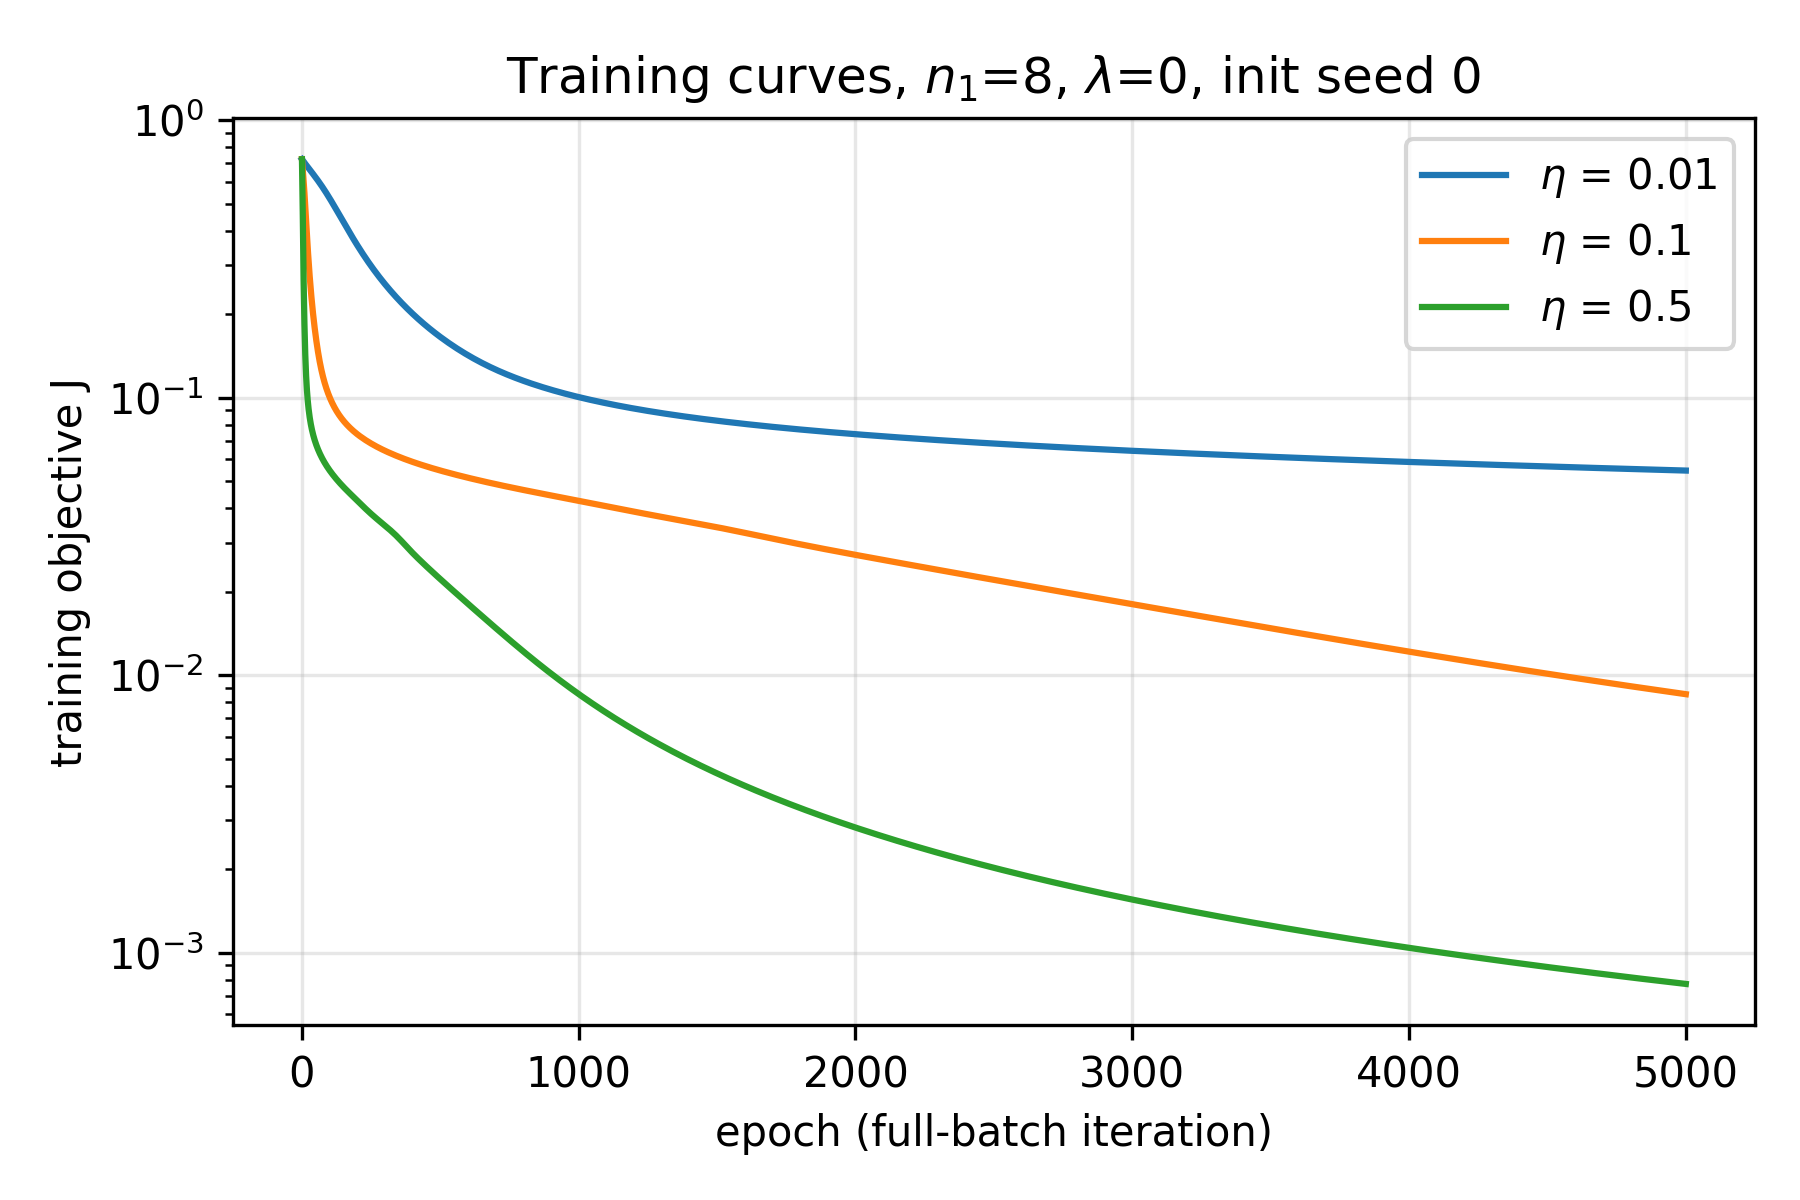
\includegraphics[width=0.85\linewidth]{../results/fig_loss_1.png}
  \caption{Training objective $J$ (logarithmic scale) against the epoch for $\eta=0.01$, $0.1$ and $0.5$. Reference configuration $n_1=8$, $\lambda=0$, initialization seed 0, which is not the selected configuration; training curves only. For all three learning rates $J$ decreases over the 5000 epochs, and at the epoch cap the curve for a larger $\eta$ lies lower.}
  \label{fig:loss}
\end{figure}

\begin{figure}[htbp]
  \centering
  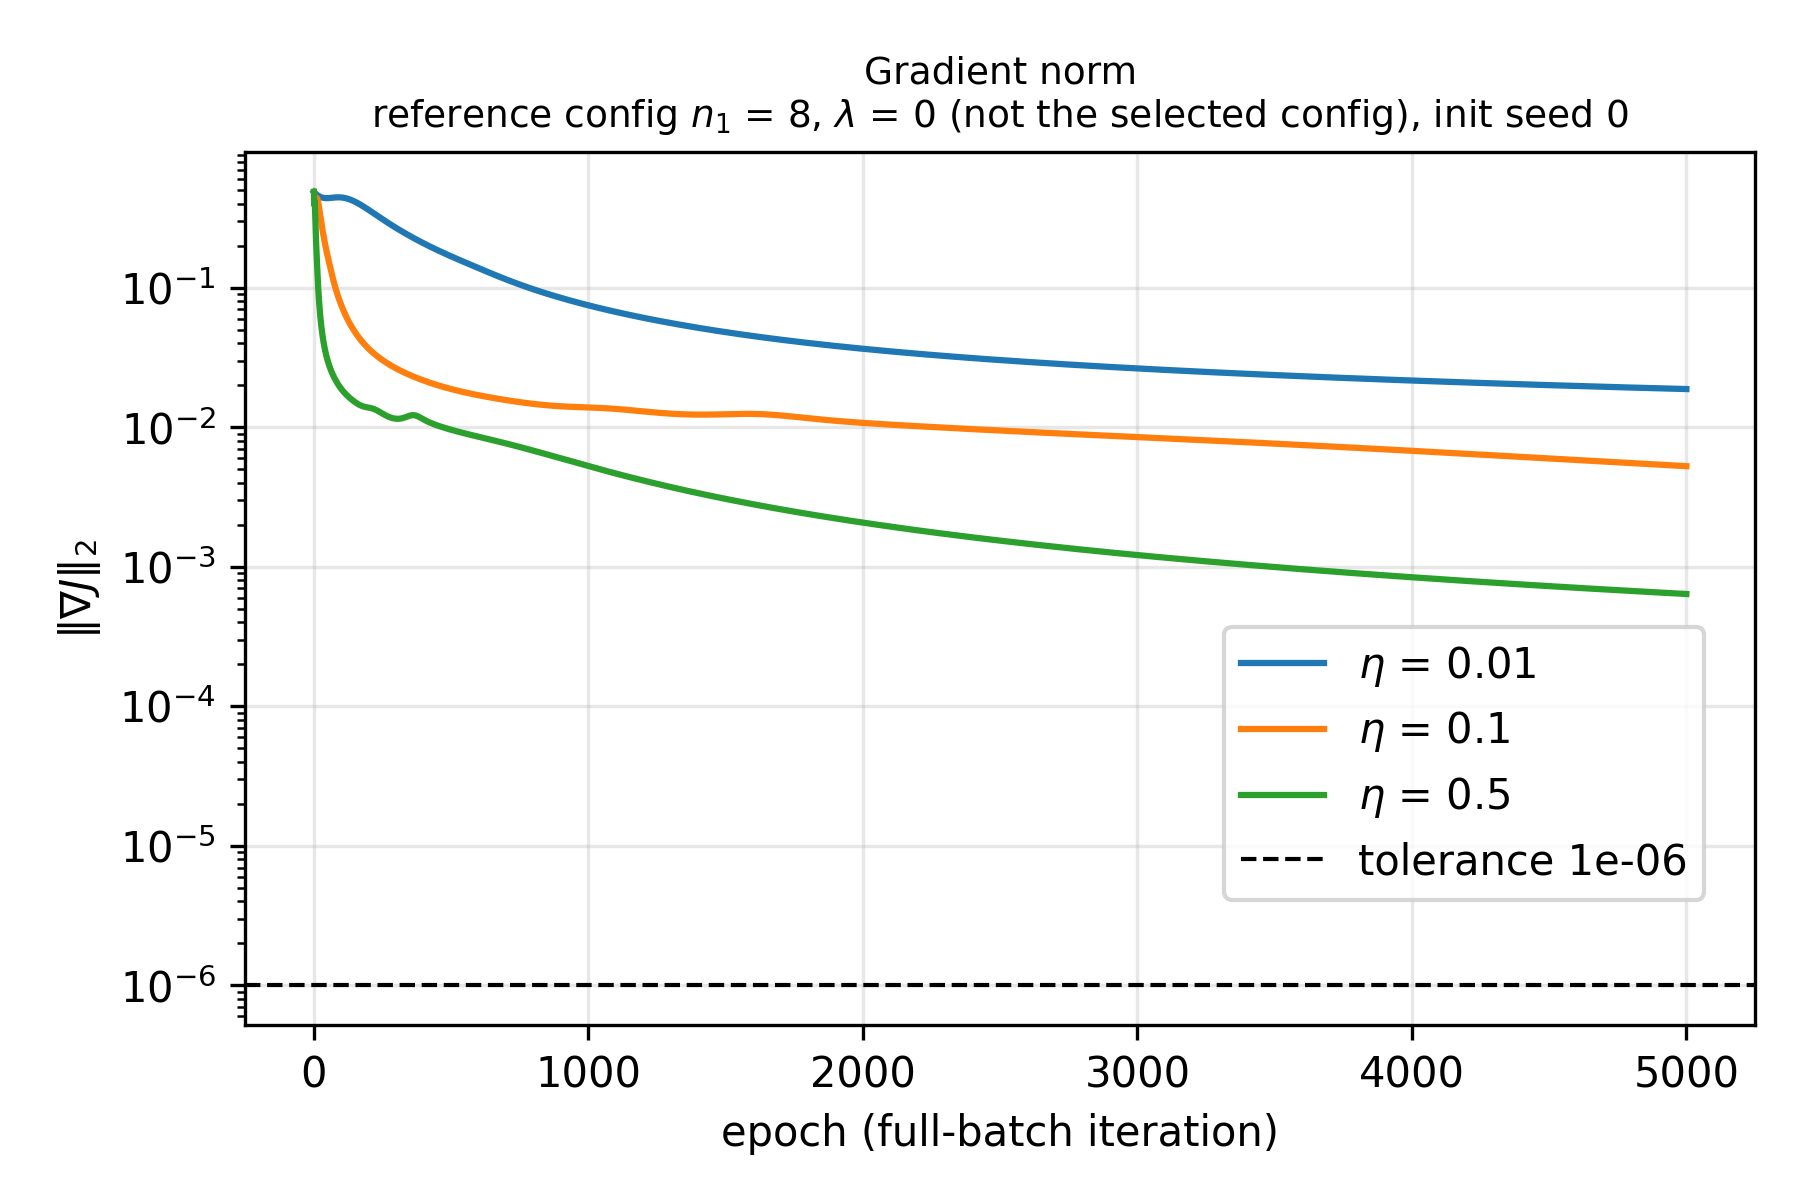
\includegraphics[width=0.85\linewidth]{../results/fig_gradnorm_2.png}
  \caption{Gradient norm $\lVert\nabla J\rVert_2$ (logarithmic scale) against the epoch for $\eta=0.01$, $0.1$ and $0.5$. Same reference configuration as Figure~\ref{fig:loss} ($n_1=8$, $\lambda=0$, seed 0; not the selected configuration); training curves only. The dashed line marks the tolerance $10^{-6}$, which none of the three curves reaches within 5000 epochs.}
  \label{fig:gradnorm}
\end{figure}

\begin{figure}[htbp]
  \centering
  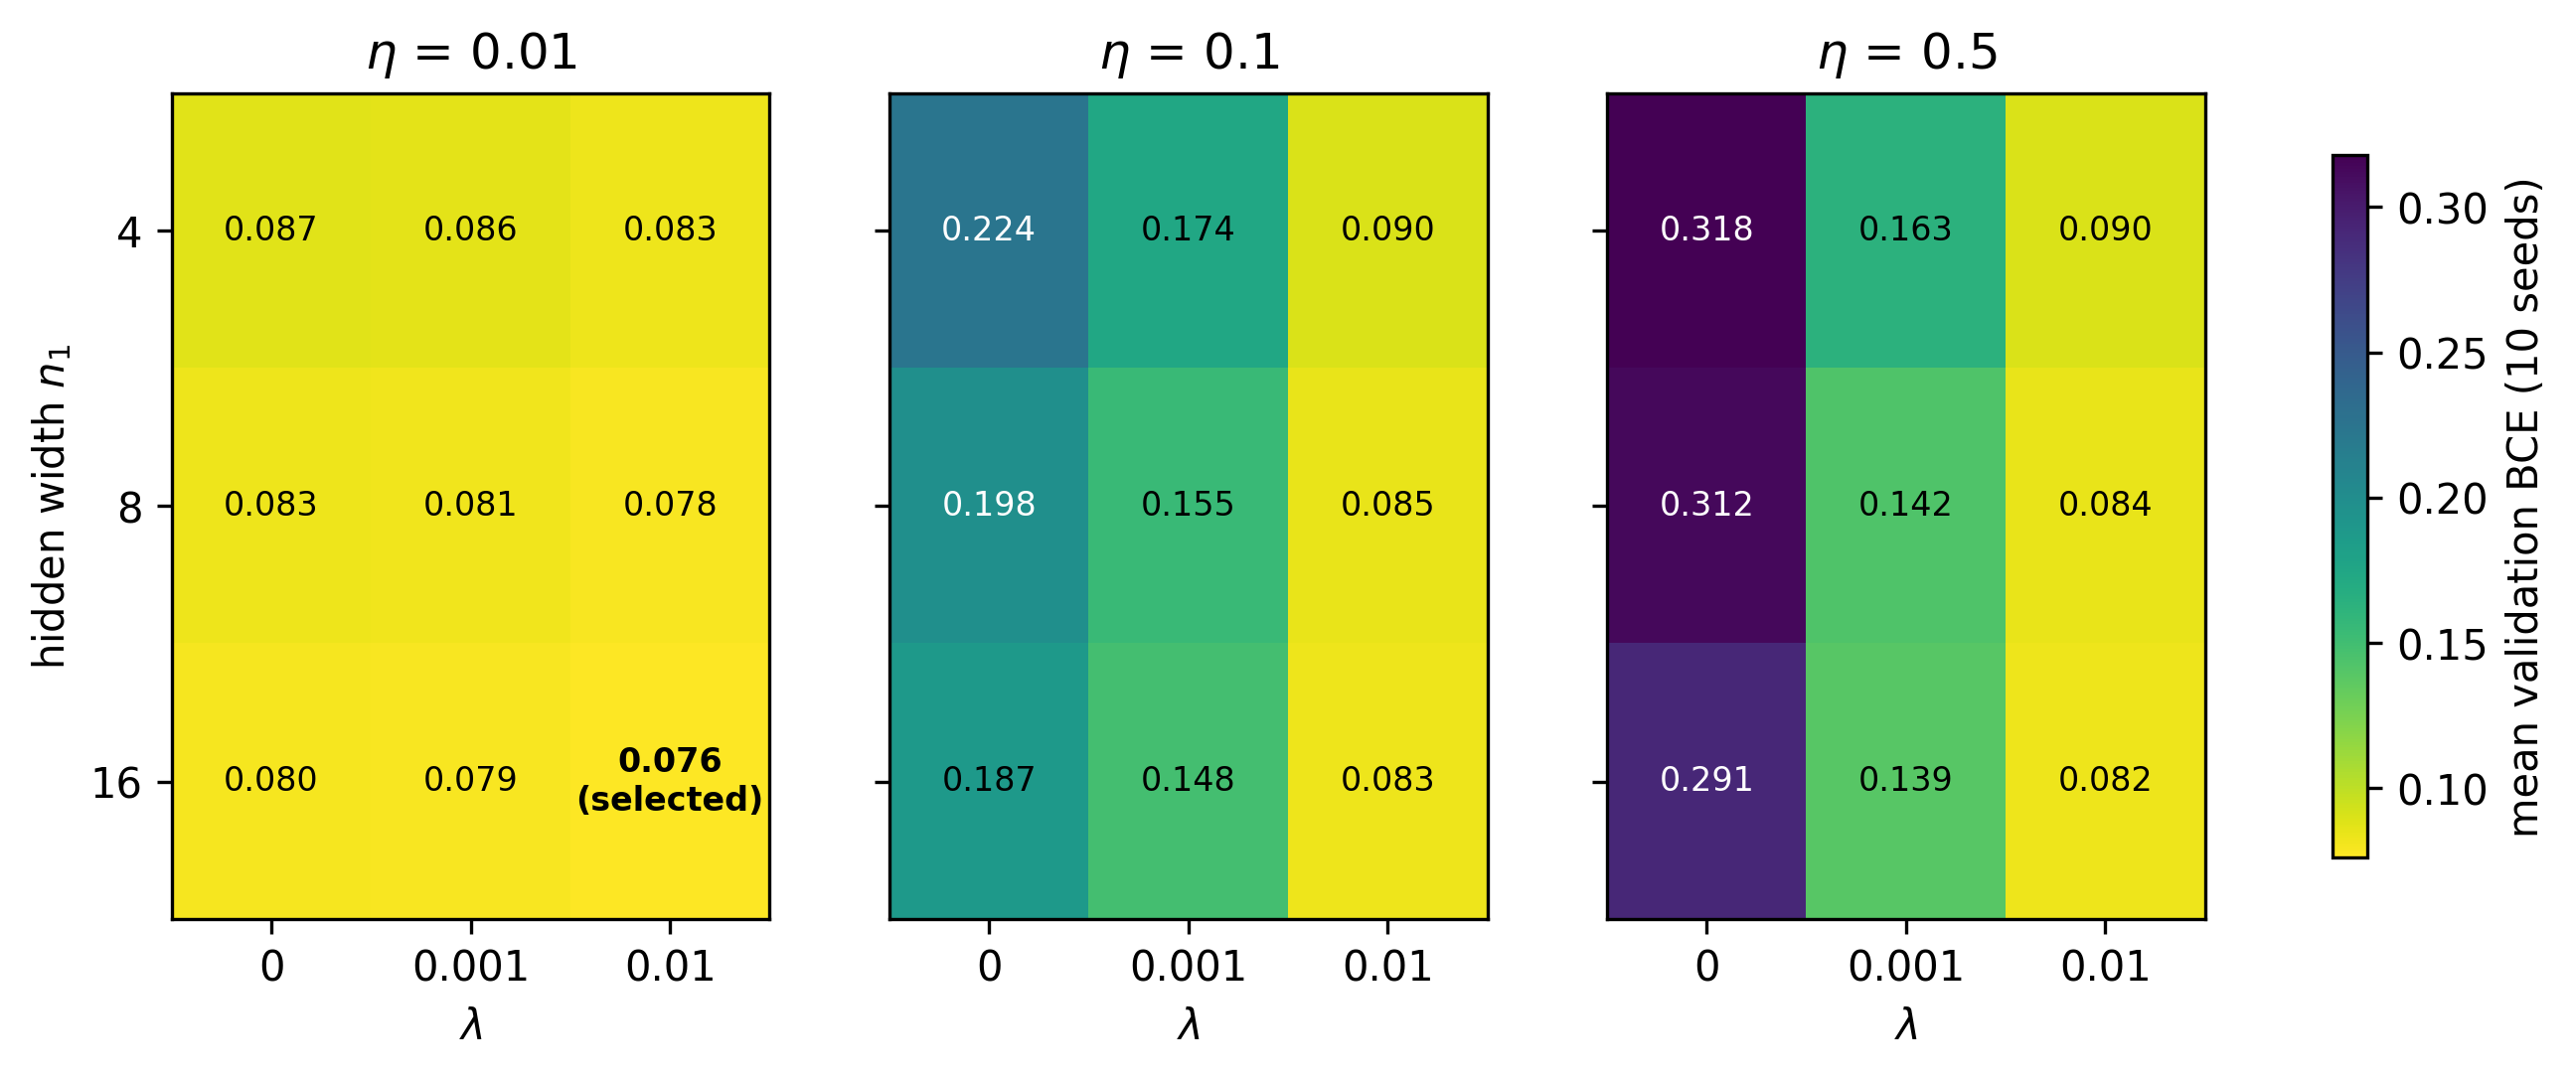
\includegraphics[width=\linewidth]{../results/fig_val_1.png}
  \caption{Mean validation BCE over initialization seeds 0--9 for each of the 27 grid cells, one panel per learning rate, with the hidden width $n_1$ on the vertical axis and $\lambda$ on the horizontal axis. The selected cell ($\eta=0.01$, $n_1=16$, $\lambda=0.01$) is marked.}
  \label{fig:val}
\end{figure}

\begin{figure}[htbp]
  \centering
  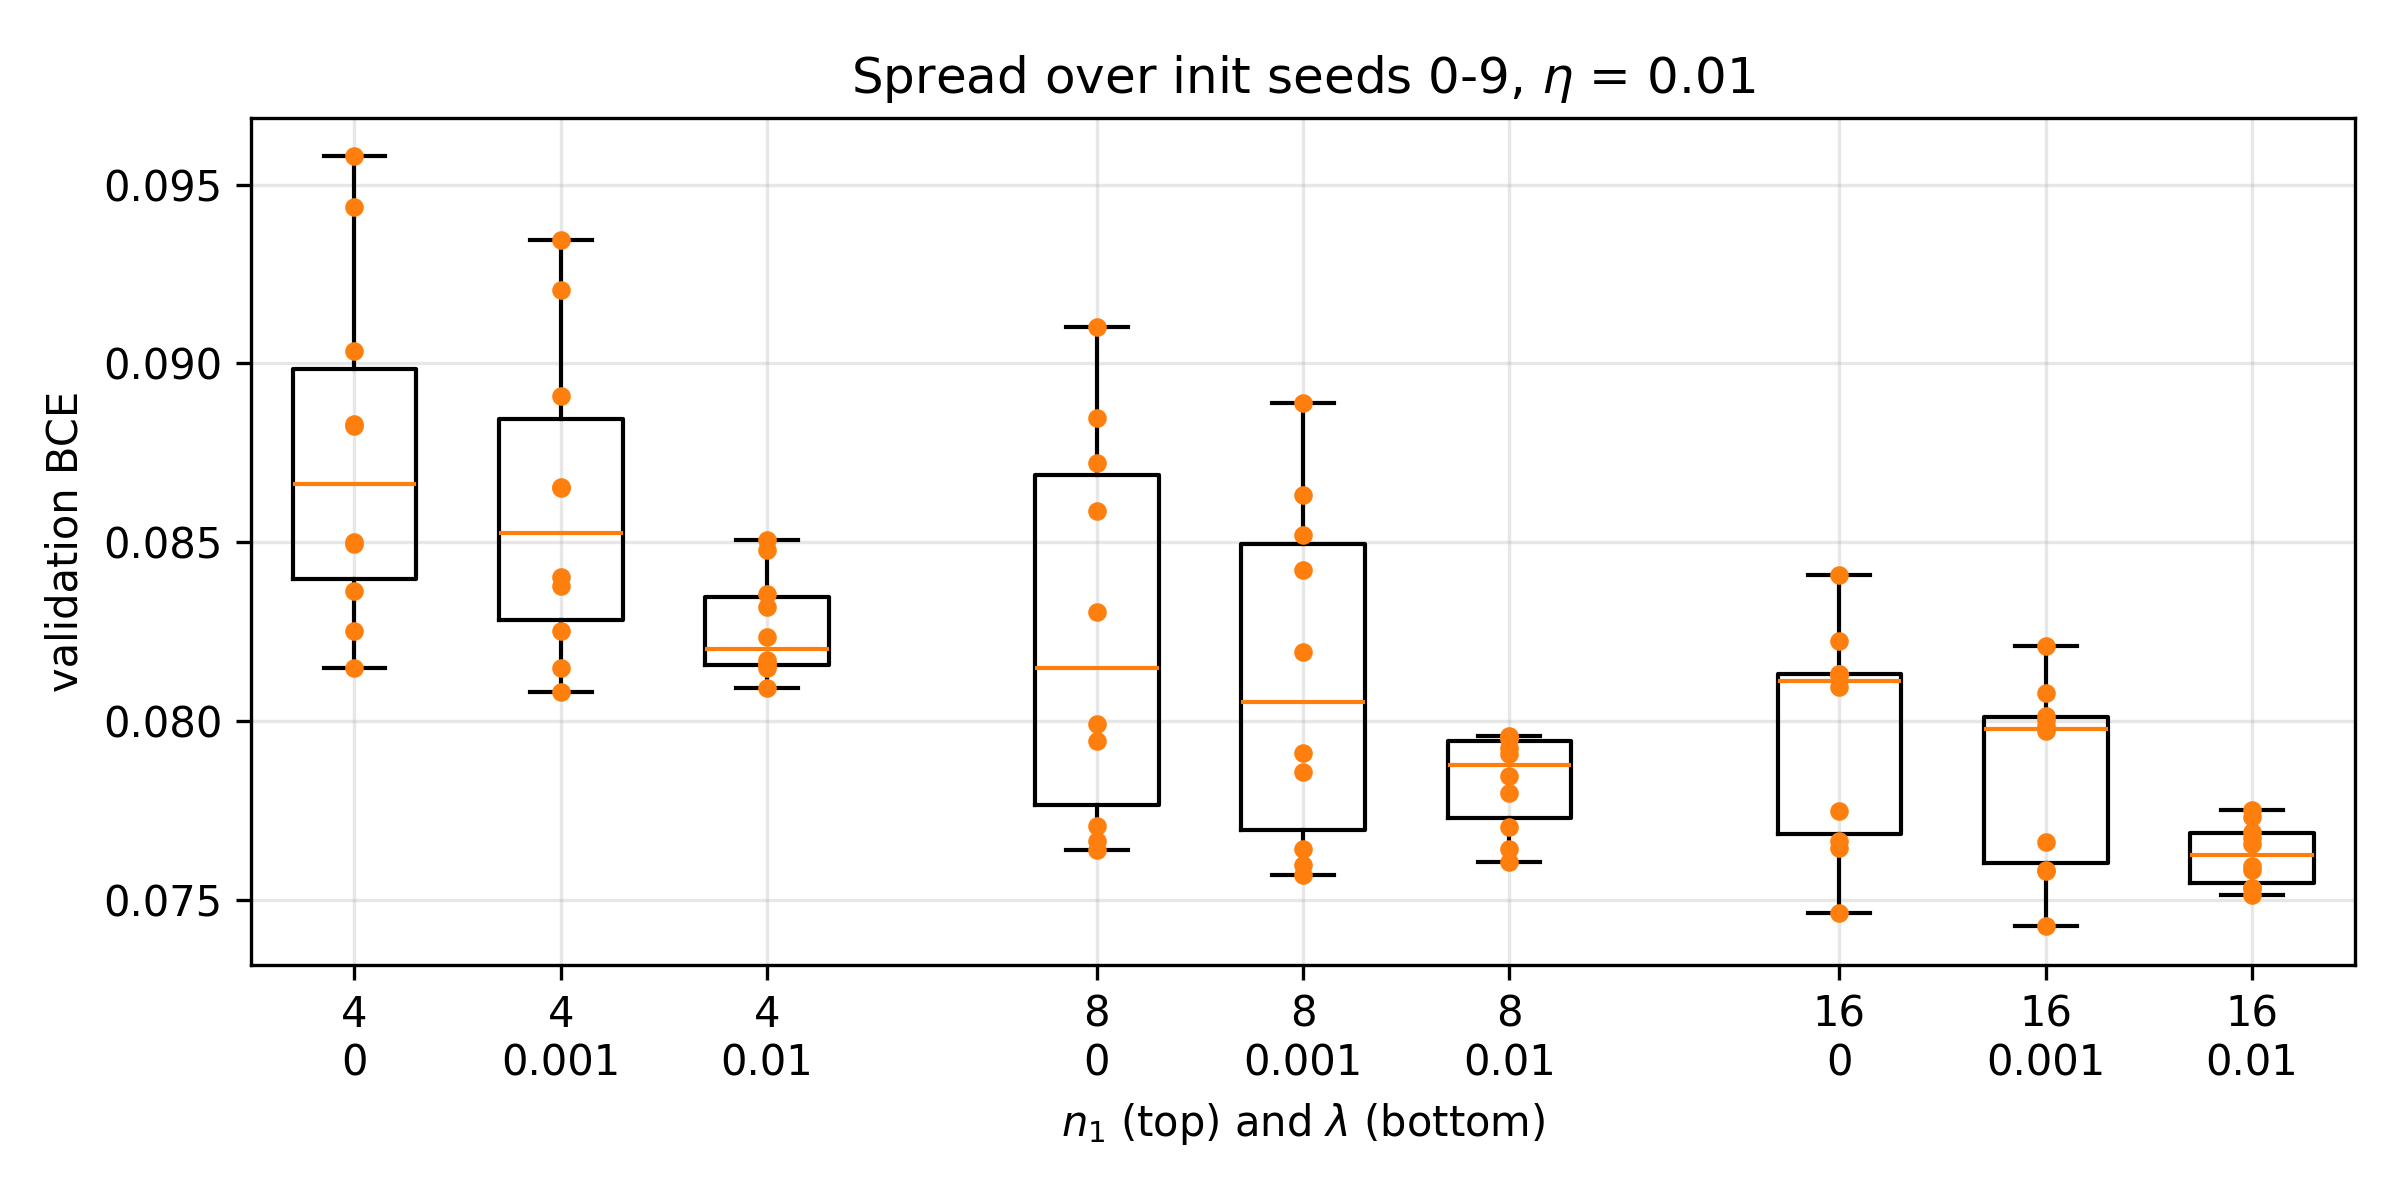
\includegraphics[width=\linewidth]{../results/fig_seeds_1.png}
  \caption{Validation BCE of the ten initialization seeds (points) and their box plots for the nine grid cells with $\eta=0.01$, labeled by $n_1$ (top) and $\lambda$ (bottom). For each hidden width, the spread over seeds is smallest at $\lambda=0.01$.}
  \label{fig:seeds}
\end{figure}

\begin{figure}[htbp]
  \centering
  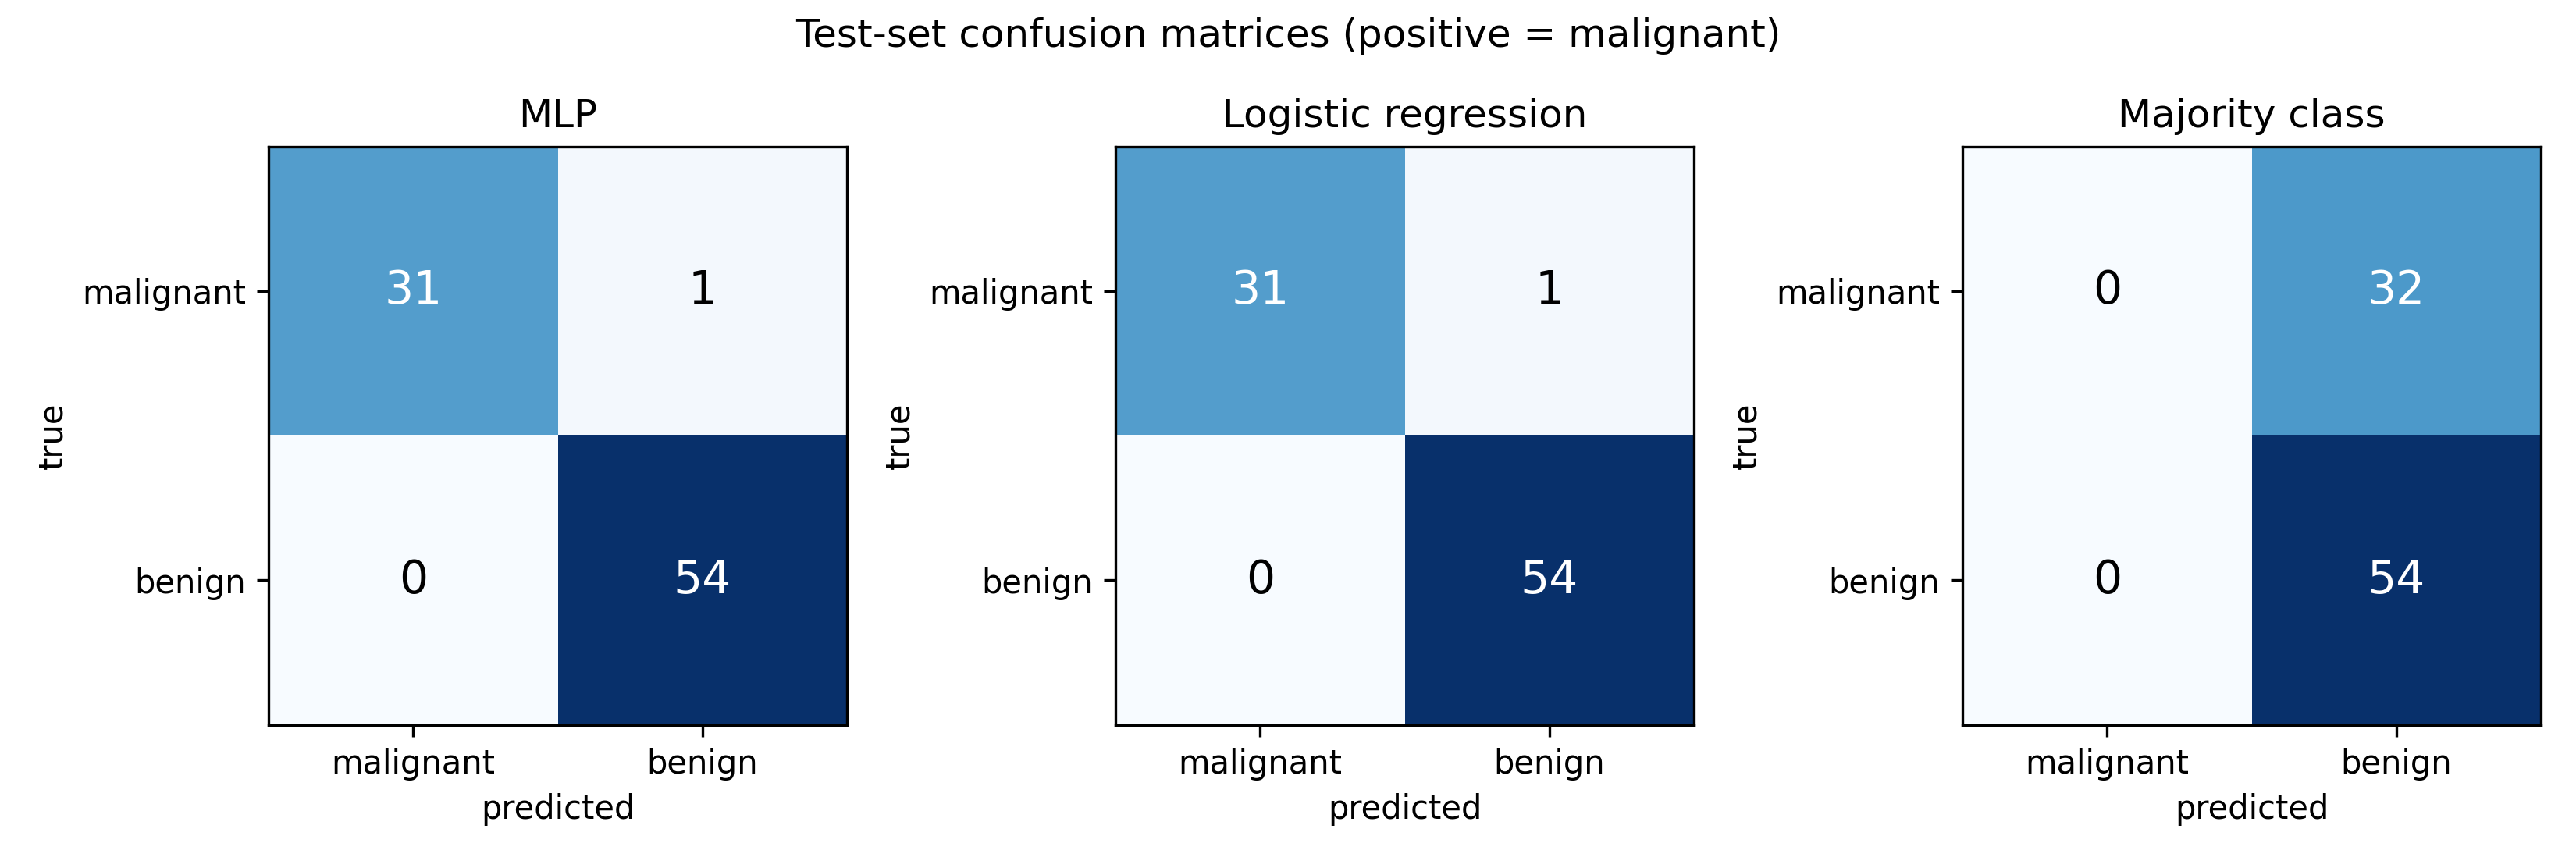
\includegraphics[width=\linewidth]{../results/fig_confusion_1.png}
  \caption{Test-set confusion matrices (positive class = malignant, threshold $0.5$) for the final MLP, logistic regression and the majority-class rule. The MLP and logistic regression have the same counts; the majority-class rule predicts benign for all 86 examples.}
  \label{fig:confusion}
\end{figure}

\begin{figure}[htbp]
  \centering
  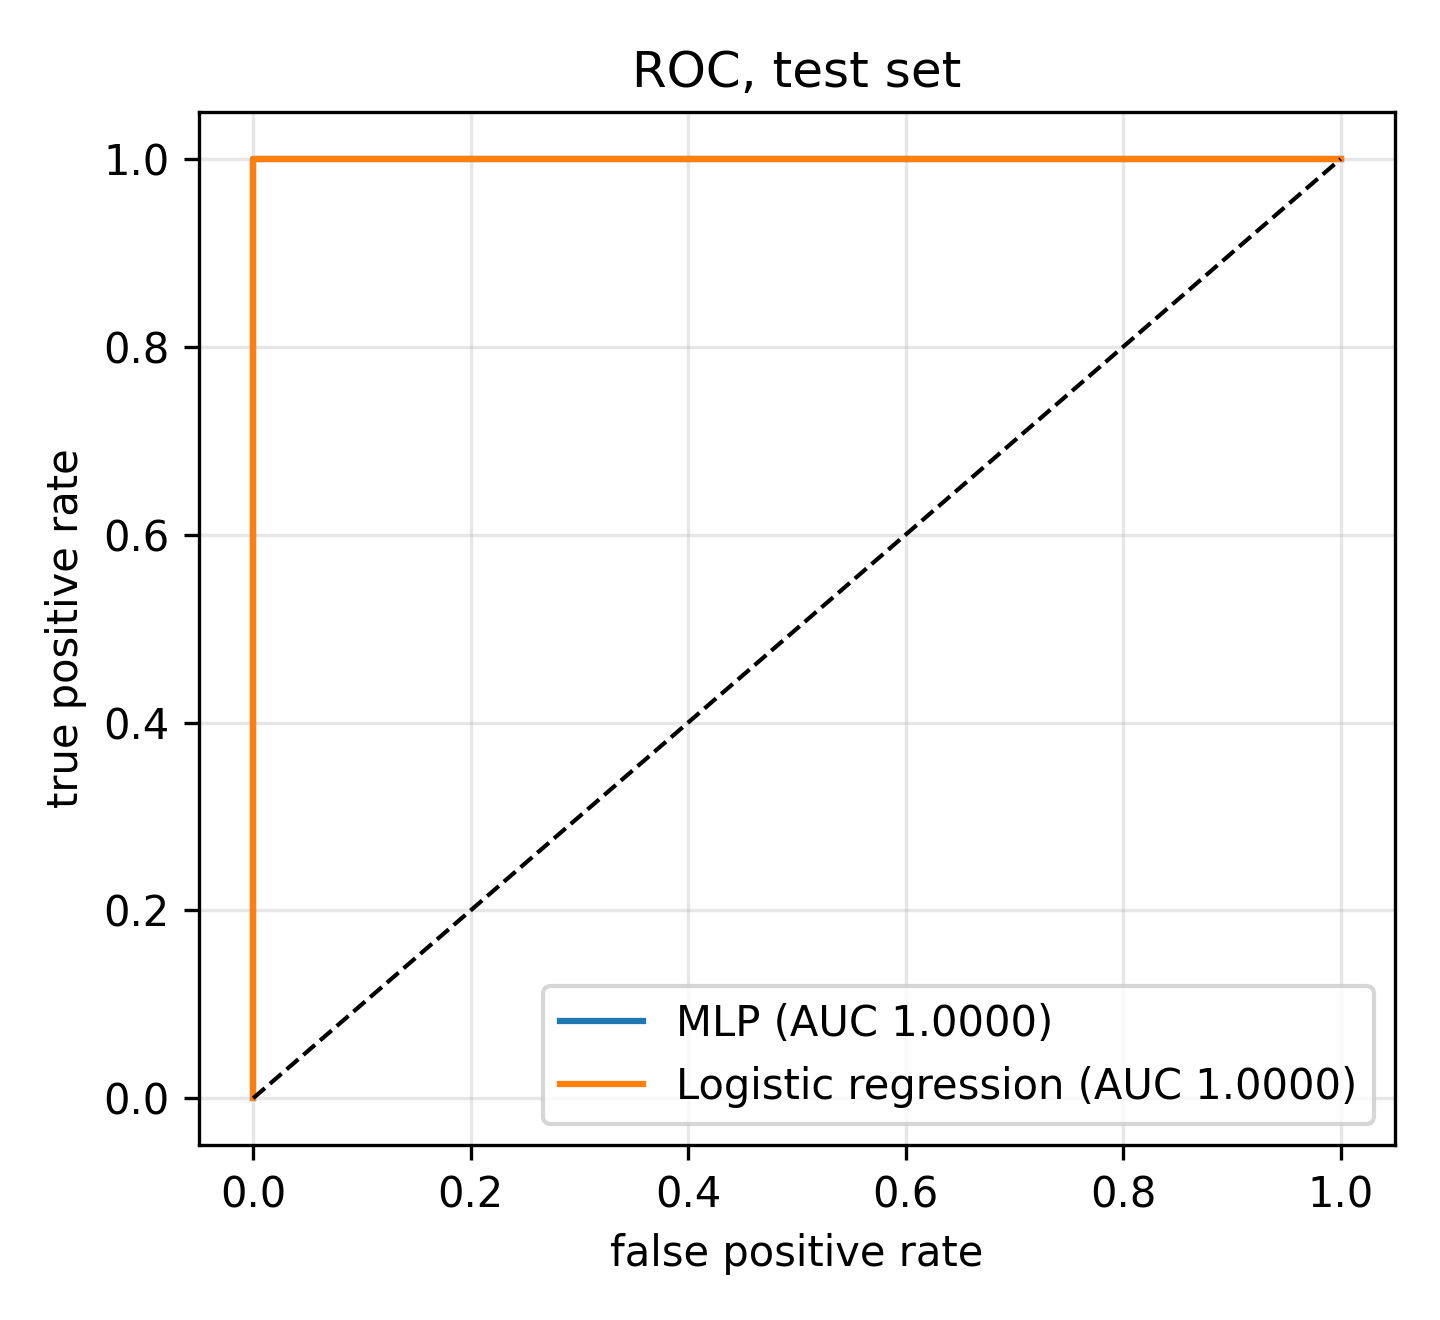
\includegraphics[width=0.6\linewidth]{../results/fig_roc_1.png}
  \caption{Test-set ROC curves of the final MLP and logistic regression; the two curves coincide and both have $\mathrm{AUC}=1.0$. An AUC of $1.0$ means a perfect ranking of the 86 test examples, not a perfect classifier: at the fixed threshold $0.5$ one malignant case is missed. The dotted diagonal corresponds to random ranking.}
  \label{fig:roc}
\end{figure}

\begin{figure}[htbp]
  \centering
  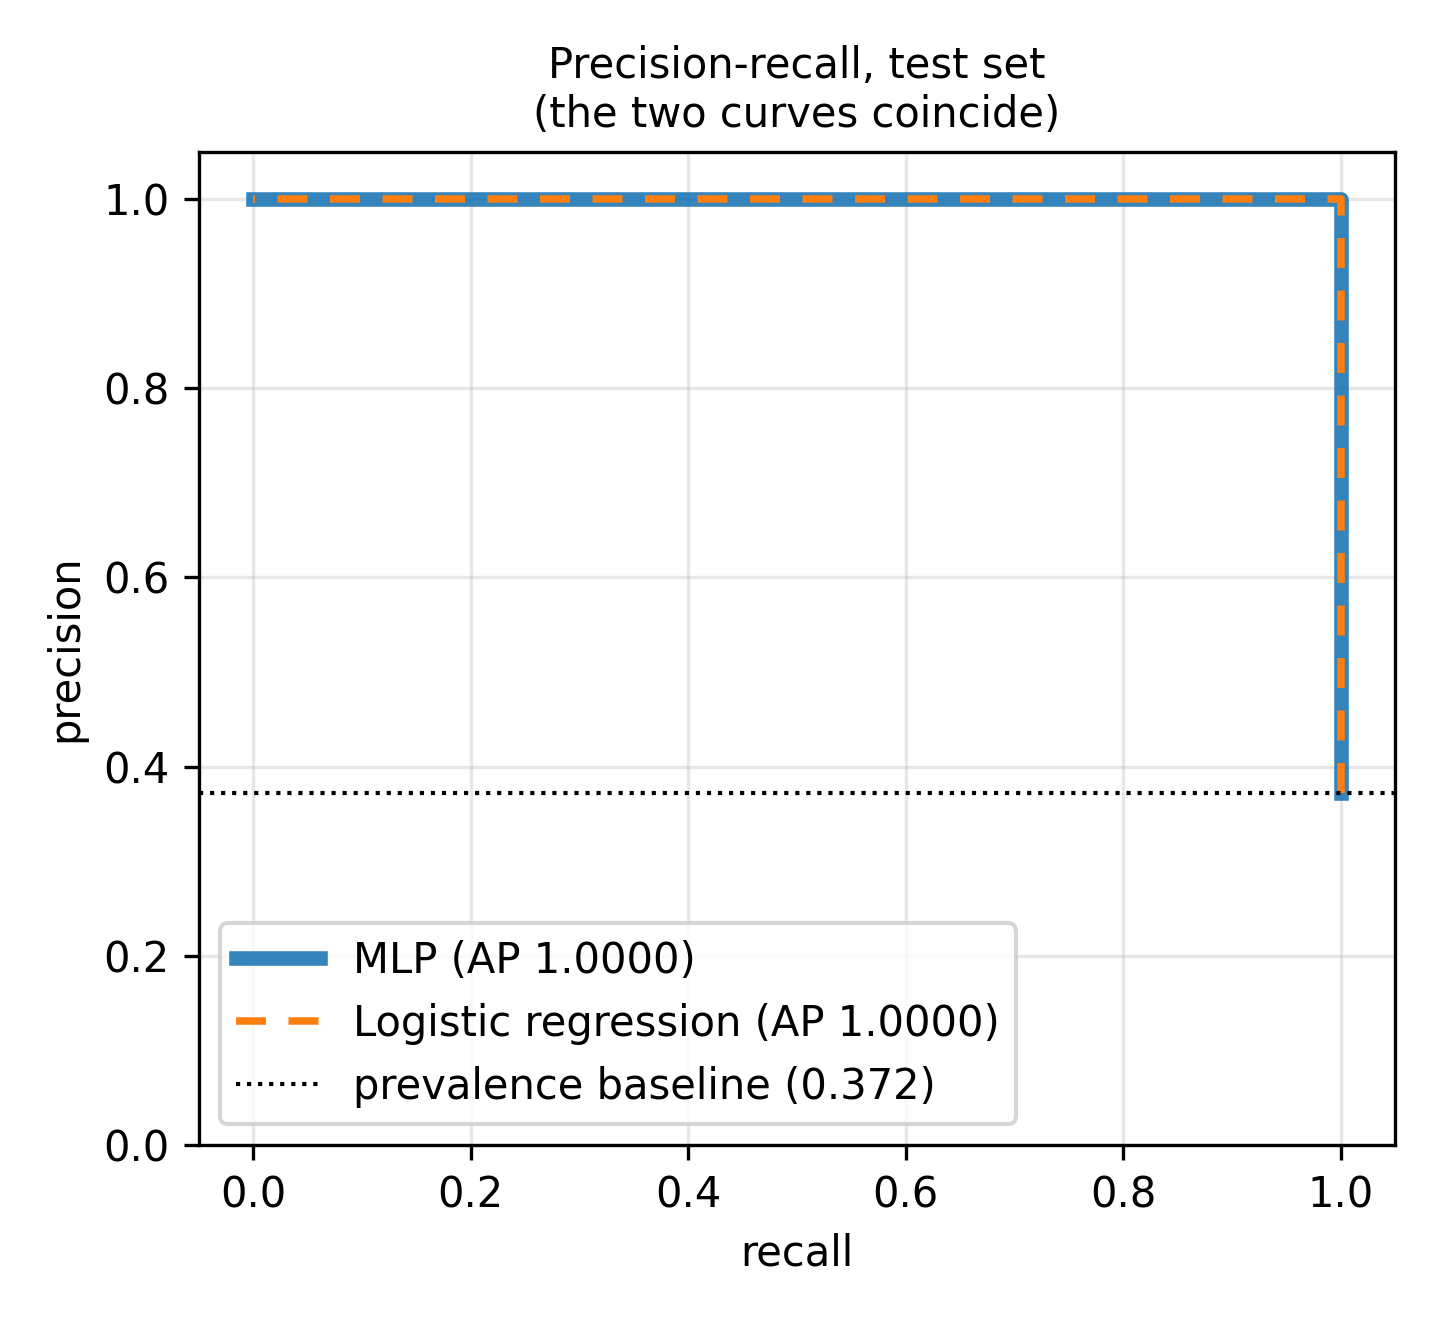
\includegraphics[width=0.6\linewidth]{../results/fig_pr_2.png}
  \caption{Test-set precision--recall curves of the final MLP and logistic regression; the two curves coincide and both have $\mathrm{AP}=1.0$. As for the ROC curve, this means a perfect ranking of the 86 test examples, not a perfect classifier: at the fixed threshold $0.5$ one malignant case is missed. The dotted line marks the fraction of malignant examples in the test set.}
  \label{fig:pr}
\end{figure}

\clearpage % place all tables and figures of Section 3.3 before Section 3.4

\subsection{Analysis and Discussion}
\label{sec:analysis}

\paragraph{Accuracy.}
On the 86 test examples the final MLP reaches an accuracy of $0.9884$, a precision of $1.0000$ and a recall of $0.9688$ (Table~\ref{tab:test}), against $0.6279$ for the majority-class rule. The single error is a false negative: a malignant mass that the model labels benign. In a screening-support setting this is the costlier kind of error, because a missed malignant case may delay follow-up, whereas a false alarm would lead to further examination. The missed case has $\hat p=0.4619$, just below the threshold $0.5$, and every malignant test example receives a higher $\hat p$ than every benign one (AUC $=1.0$). The ranking of the scores is therefore perfect on this test set, and the error comes from the fixed threshold. The threshold was not tuned.

\paragraph{Convergence and stability.}
In the reference configuration ($n_1=8$, $\lambda=0$, seed 0), the objective starts at $J=0.7230$ and decreases for all three learning rates. After 5000 epochs it is $0.054615$ for $\eta=0.01$, $0.008543$ for $\eta=0.1$ and $0.000772$ for $\eta=0.5$, with gradient norms $0.018799$, $0.005266$ and $0.000639$. A larger learning rate thus reaches a lower training objective within the same number of epochs, and none of the three runs diverged or reached the tolerance $10^{-6}$. The validation error tells a different story. With $\lambda=0$, the mean validation BCE rises with the learning rate, for example for $n_1=8$ from $0.08250$ at $\eta=0.01$ to $0.19755$ at $\eta=0.1$ and $0.31228$ at $\eta=0.5$. For $n_1=8$ and $\eta=0.5$ the mean training BCE is $0.00080$ against a validation BCE of $0.31228$. A training error far below the validation error is consistent with overfitting; this was not tested directly. Regularization narrows the gap: at $\eta=0.5$ and $\lambda=0.01$ the training BCE is $0.05715$ and the validation BCE $0.08441$, and the validation BCE over the three widths lies in $0.0825$--$0.0898$ for $\eta=0.1$ and $0.0824$--$0.0898$ for $\eta=0.5$, close to the range $0.0763$--$0.0826$ at $\eta=0.01$. The mean validation accuracy varies much less than the BCE, from $0.9471$ in the weakest cell to $0.9765$ for the selected configuration. The selected model did not reach the tolerance: it stopped at the 5000-epoch cap with $\lVert\nabla J\rVert_2=0.015658$, and only 6 of the 270 grid runs (all with $\eta=0.5$, $n_1=4$, $\lambda=0.01$) satisfied $\lVert\nabla J\rVert_2<10^{-6}$ before the cap.

\paragraph{Computational cost.}
The selected network has $P=513$ parameters (\eqref{eq:wdbc-params}; $129$ and $257$ for $n_1=4$ and $8$). Each epoch is one forward and one backward pass over the 398 training examples, and a run is limited to 5000 epochs. The grid consists of 270 such runs.

\paragraph{Comparison with the baseline.}
The MLP and logistic regression make the same single error (confusion counts $31/0/54/1$) and share all threshold-based metrics. The MLP has the lower test log loss, $0.0497$ against $0.0610$, but this is a difference between two values computed on 86 examples from one split, without an estimate of its uncertainty. We therefore claim no difference in quality between the two models. On this split, the added hidden layer did not change the classification of any test example relative to a linear model.

\paragraph{Limitations.}
The study uses one dataset of 569 samples, one split with 85 validation and 86 test examples, and no external validation. The data file has no patient identifiers, so a patient-level split was not possible, and the assumption that the examples are independent is not verified. The selected configuration sits on the edge of the grid on all three axes, so a setting with lower validation error may lie outside the grid. In addition, the small learning rate combined with the epoch cap may act like early stopping, because training ends while $J$ is still decreasing; part of the validation advantage of $\eta=0.01$ may therefore come from this. This is a possibility, not a tested explanation. The final model was evaluated once on the test set; a later seed-sensitivity check on the test set did not change it and was not used for any decision. In that check every initialization seed gave the same confusion counts $31/0/54/1$ and the test log loss ranged from $0.04864$ to $0.05022$, so the test result did not change across the ten seeds tried. Finally, this is an educational model and not a diagnostic tool; the results support no clinical claim.
